\documentclass[11pt]{jreport}
\usepackage{wuse_thesis}
\usepackage{indentfirst}
\usepackage{url}	% \url{}コマンド用.URLを表示する際に便利
\usepackage{otf}
\usepackage{xcolor}
\usepackage[dvipdfmx]{graphicx}
\usepackage{float}
\usepackage{amsmath} 
\usepackage{listings}
\lstset{
    basicstyle=\ttfamily\small,
    breaklines=true,
    showstringspaces=false,
    frame=single,
    numbers=left,
    numberstyle=\tiny,
    tabsize=4
}
\usepackage{xcolor}
\lstset{
    keywordstyle=\color{blue},
    commentstyle=\color{green!60!black},
    stringstyle=\color{red}
}
\newcommand{\todo}[1]{\colorbox{yellow}{{\bf TODO}:}{\color{red} {\textbf{[#1]}}}}
\newcommand{\change}[1]{\colorbox{green}{{\bf CHANGE}:}{\color{red} {\textbf{[#1]}}}}
\newcommand{\colorer}[1]{\colorbox{red}{{\textbf{[#1]}}}}

\newcommand{\RQone}{ソースコードを自動生成できるコメントで提示する情報の種類は何か}
\newcommand{\RQtwo}{ソースコードを自動生成できるコメントの情報量はどの程度か}
%%%%%%%%%%%%%%%%%%%%%%%%%%%%%%%%%%%%%%%%%%%%%%%%%%%%%%%%%%%%%%%%%%%%%%%%

%%
%% 主に表紙を作成するための情報
%%

%%  タイトル(修論の場合は英語表記も指定)
 % \title{ソースコードを自動修正可能なレビュー指摘の分析}
 \title{コードレビューコメントの特徴による\\ソースコード自動修正の精度の比較}
%\etitle{Test\\Test\\Test}

%%  著者名(修論の場合は英語表記も指定)
\author{赤松 汰輝}
%\eauthor{Akinori Ihara}

%% 卒業論文・修士論文(以下のどちらかを選択)
\bachelar	% 卒業論文(4年生用)
%\master  	% 修士論文(M2用)

%%  学科・クラスタ
\department{システム工}
%\department{デザイン情報}
%\department{デザイン科学}

%%  学生番号
\studentid{60266003}

%%  卒業年度
\gyear{2024}		% 提出年が2022年なら,2021年度

%%  論文提出日
\date{2025年2月12日}	% 修士の場合は月(2021年2月)までとし,英語表記も指定
%\edate{February 2021}	% 修士の場合,こちら(英語表記)も有効化

%%%%%%%%%%%%%%%%%%%%%%%%%%%%%%%%%%%%%%%%%%%%%%%%%%%%%%%%%%%%%%%%%%%%%%%%

\begin{document}

\maketitle

%%
%%  概要
%%
\begin{abstract}

\end{abstract}

%%  目次
\tableofcontents

%%  図目次 (図目次をいれたければ以下のコメントをはずす)
%\listoffigures

%%  表目次 (表目次をいれたければ以下のコメントをはずす)
%\listoftables

\newpage
\pagenumbering{arabic}	% 以降のページ番号を算用数字に

%%%%%%%%%%%%%%%%%%%%%%%%%%%%%%%%%%%%%%%%%%%%%%%%%%%%%%%%%%%%%%%%%%%%%%%%

%%
%%  本文はここから
%%

\chapter{はじめに}
近年ソフトウェア開発はソフトウェアの大規模化や複雑化により,個人で行うのではなく,複数人で行うことが主流になっている.その中で,ソースコードレビュー(以後,コードレビュー)とはソフトウェア開発において複数の開発者が協力して行う品質管理活動の一つであり,開発者(実装者)が機能追加,不具合修正のために変更したソースコードを,自身を除く開発者(レビューア)が検証する作業である.特に,検証作業を複数人のレビューアが取り組むことで,ソースコードの品質が向上する[1]\todo{参考文献設定}.

大規模なプロジェクトでは1ヶ月に数百件以上の検証依頼があり,これらを効率的に処理するためにはレビューアが指摘を正確かつ簡潔に実装者に伝え,コミュニケーションの回数を少なく抑えることが期待される[2]\todo{参考文献設定}.従来研究によると,レビューアと実装者のコミュニケーションにおいて,レビューアの意図が正確に伝わらないケースが多く発生している.具体的には,レビューアが指摘した問題に対する修正方針が曖昧な場合や,実装者が指摘の背景にある設計意図を理解できていない場合などがある.その結果,実装者が意図を確認するための質問や,レビューアが追加で説明を行うといった複数回のやり取りが必要となり,レビュー完了までの時間が長期化する傾向にある\todo{参考文献設定}.さらに,この問題はレビューアと実装者が異なるタイムゾーンで作業している場合や,非同期でコミュニケーションを行う必要がある場合に特に顕著となる.このような課題に対して,レビューアの指摘を正確に解釈し,適切なコード修正を自動的に提案する手法が求められている.

従来研究では,コードレビューにかかるコスト軽減を目的に,変更されたソースコードとそれに対するレビューアからの指摘コメントを入力とし,ソースコードを自動修正するモデルを開発している [3]\todo{参考文献設定}.従来研究の手法はコードレビューの指摘に基づき自動修正を実現している.しかし,レビューアからの指摘コメントに含まれる情報の種類や情報量によって精度にばらつきが見られた.従来研究ではレビューコメントの情報の種類や量がコード自動修正の精度に与える影響までは分析されていない.
本研究では,レビューコメントの特徴を分析することで,レビューアが意図していたソースコードをモデルが生成できるレビューコメントの特徴を明らかにする.具体的には,2つのResearch Question(RQ)に回答する.
\begin{itemize}
\item RQ1:\RQone
\item RQ2:\RQtwo
\end{itemize}
RQ1では従来研究のレビューコメントで提示されている情報の種類に関するラベルづけを行うことで,情報の種類によるモデルの精度を分析する.RQ2ではレビューコメントの情報量と自動修正の精度の関係を調査するためレビューコメントに関連情報を追加し,情報を補強したレビューコメントをモデルに入力した場合の精度を比較評価する.
以降,本論文では,2章で本研究の対象であるコードレビューと従来研究,本研究の位置付けを述べ,3章ではソースコードの規模が本研究で用いる評価指標であるcodeBLEUスコアに与える影響を述べる.続く4,5章では,設定したRQにおけるそれぞれの提案手法と結果,考察を述べ,6章では,妥当性の脅威を述べ,最後に7章で本研究をまとめる.

\chapter{コードレビュープロセス}\label{chap:fig-tab-exp}
\section{コードレビュー}
コードレビューは,ソフトウェア開発フローの中の1つであり,開発者(実装者)が作成,変更したソースコードの導入可否を判断するために別の開発者が検証することである.従来のコードレビューは,開発者が一堂に会して行う対面形式が主流であった.このような形式は正式なインスペクションとも呼ばれ,特定の時間と場所で複数の開発者が集まり,詳細なレビューを実施する.

しかし,近年ではより軽量で柔軟なコードレビュー手法である「モダンコードレビュー」が普及している.モダンコードレビューは,開発者がコードを変更するたびに行う非同期かつ非公式なレビュープロセスであり,オンラインツールを活用して実施される.この手法は,開発の迅速性を保ちながら,継続的にコードの品質を維持することを可能にする.
現在のモダンコードレビューは,GitHubのプルリクエスト(Pull Request: PR)機能を用いて行われることが多い.

プルリクエストは,開発者が作成したソースコードの変更を本番環境に反映する前に,その変更内容をレビュー担当者に確認を依頼する仕組みである.実装者はまず新しい機能の追加やバグ修正のために,メインブランチから作業用ブランチを作成する.その後,作業用ブランチで必要な変更を加え,プルリクエストを作成する.レビュー担当者は,プルリクエストで示された変更内容について,コーディング規約への準拠,バグや潜在的な問題の有無,設計の適切性,パフォーマンスへの影響,セキュリティ上の懸念などの観点からレビューを行う.問題を発見した場合はコメントを付けて修正を依頼し,実装者は指摘された箇所を修正して再度レビューを依頼する.最終的にレビュー担当者が承認すると,変更内容がメインブランチにマージされる.

このようなコードレビューを行うことで,ソースコードのバグの混入率が低下する\todo{参考文献設定}というだけでなく,開発者間での知識伝達が促進され,コードの品質と保守性が向上するという利点もある.また,チーム内でのベストプラクティス(例えば,コードの再利用性を高めるためのデザインパターンの適用方法や,パフォーマンスを考慮したアルゴリズムの実装方法,セキュリティを考慮した入力値の検証方法など)の共有が進む.さらに,新人開発者にとっては,プロジェクト固有の設計思想やコーディング規約,テスト方針,さらにはチームで採用している技術スタックの効果的な使用方法などを学ぶ教育機会としても機能する.

しかし,コードレビューにはいくつかの課題も存在する.実装者にとっては,レビュー待ち時間により開発作業が停滞し,機能のリリースが遅延するという問題がある.また,レビュー担当者は自身の開発作業に加えてレビュー作業も行う必要があり,作業負荷の増加によって本来の開発タスクに支障が出る可能性がある.これらの問題は,プロジェクト全体のスケジュールにも影響を与え,製品の市場投入の遅れにもつながりうる.また,レビューコメントの解釈に齟齬が生じた場合は,追加のコミュニケーションが必要となり,さらなる時間的コストが発生する.特に大規模なプロジェクトでは,膨大なレビュー件数の管理も大きな課題となっている.

\section{従来研究}
コードレビューの自動化に関する研究として,Tufanoらの研究\todo{参考文献設定}が挙げられる.この研究では,以下の2つのタスクを対象にDeep Learningモデルによる自動化を試みている:

1つ目は,コードレビュー提出前のフィードバック生成である.開発者が提出したコード($C_s$)に対して,レビュアーが指摘するであろう修正を実装したコード($C_r$)を自動生成する.これにより,開発者は正式なレビュー前に潜在的な問題点を把握できる.

2つ目は,レビュアーのコメントに基づくコード修正の自動化である.開発者が提出したコード($C_s$)とレビュアーのコメント($R_{nl}$)を入力とし,そのコメントに対応した修正を実装したコード($C_r$)を生成する.これにより,レビュアーは具体的な修正例を開発者に示すことができる.

従来研究では,GitHubおよびGerritのリポジトリから約17,000件の $\langle C_s, R_{nl}, C_r \rangle$ の三つ組データを収集し,エンコーダ-デコーダモデルを用いて評価を行った.1つ目のタスクでは1つの予測で3\%,10個の予測では16\% の正解率を達成した.2つ目のタスクでは1つの予測で12\%,10個の予測では31\% の正解率を達成している.

\section{動機}
本研究では,前章で述べたように,レビューコメントの特徴を分析することで,レビューアが意図していたソースコードをモデルが生成できるようなレビューコメントを明らかにすることを目的とする.

従来研究では,コードレビューの自動化において一定の成果を示しているものの,レビューアからの指摘コメントに含まれる情報の種類や情報量によって精度にばらつきが見られた.実際のコードレビューでは,レビューアは様々な形式や詳細度でコメントを記述している.例えば,「変数名を修正する」という簡潔なコメントと,「変数名をfooからbarに変更し,クラス全体での命名規則に従うようにする」という具体的なコメントでは,モデルの生成精度に差が生じる可能性がある.

このような背景から,本研究では以下の2つのResearch Question(RQ)を設定し,レビューコメントの特徴がコード生成の精度に与える影響を分析する:

\begin{itemize}
   \item RQ1: \RQone
   \item RQ2: \RQtwo
\end{itemize}

これらの分析を通じて,効果的なレビューコメントの特徴を明らかにし,コード生成モデルの精度向上に向けた知見を得ることを目指す.これにより,コードレビューの自動化における精度向上だけでなく,人手によるコードレビューの質の向上にも貢献することが期待される.

\chapter{事前分析}\label{chap:fig-tab-exp}

\section {codeBLEUスコア}

codeBLEUスコアとは,自然言語処理(NLP)の分野,特にコード生成タスクにおいて使用される評価指標である.従来機械翻訳の評価には生成データと正解データ完全一致している割合やN-gramが用いられてきた.しかし,完全一致では正解データと類似度の高いデータを生成できても十分に評価されない.また,N-gramでは単語の並び順や文の構造については評価できるが,文法的な意味や論理的な意味まで考慮できない.そこで近年では機械翻訳タスクの評価にはBLEUスコアというものが用いられる.

\begin{displaymath}
\text{BLEU} = BP \cdot \exp\left(\sum_{n=1}^{N} w_n \log(p_n)\right)
\end{displaymath}

\noindent
ただし,

\begin{displaymath}
BP =
\begin{cases} 
1 & (c > r) \\ 
e^{1 - r/c} & (c \leq r)
\end{cases}
\quad
\begin{aligned}
&c: \text{生成文の長さ} \\
&r: \text{正解文の長さ}
\end{aligned}
\end{displaymath}

\vspace{1em}

\begin{displaymath}
p_n = \frac{\sum_{i} \text{生成文 }i \text{ と正解文 }i \text{ で一致した } n\text{-gram の数}}{\sum_{i} \text{生成文 }i\text{ の } n\text{-gram の総数}}
\end{displaymath}

\vspace{1em}

\begin{displaymath}
w_n = \frac{1}{N}
\end{displaymath}

BLEUスコアを採用することで部分的な一致も評価に含めることで,意味的に正しい異なる実装も適切に評価でき,また複数のN-gramスコアを組み合わせることで,局所的な類似性だけでなく,より広い文脈での類似性も評価できる.

BLEUスコアを用いると自然言語間の類似度を包括的に評価できるが,ソースコードを評価する際にはソースコードが持つ特徴を十分に考慮できないという課題がある.具体的には,ソースコードは自然言語に比べ使用される単語の種類が少ないため直感的な一致度よりもスコアが高くなってしまったり,自然言語のようなシーケンシャル構造ではなくツリー構造を持っているためN-gramでは類似度を正しく評価できない.また,異なる実装方法でも同じ結果を得られるというコードの意味的同値性や,各プログラミング言語に固有のAPIの使用規則についても考慮できない.

これらのようなソースコード間の類似度を評価できない課題を対応するために,以下の4つの要素を考慮した評価を行えるcodeBLEUスコアを用いる.

\begin{displaymath}
\text{CodeBLEU} = \alpha \cdot \text{BLEU} + \beta \cdot \text{BLEU}_{\text{weight}} + \gamma \cdot \text{Match}_{\text{ast}} + \delta \cdot \text{Match}_{\text{df}}
\end{displaymath}

\noindent
ただし,
\begin{align*}
&\alpha, \beta, \gamma, \delta: \text{重み係数(}\alpha + \beta + \gamma + \delta = 1\text{)} \\
&\text{BLEU}: \text{通常のBLEUスコア} \\
&\text{BLEU}_{\text{weight}}: \text{言語固有のキーワードに基づく重み付きBLEUスコア} \\
&\text{Match}_{\text{ast}}: \text{抽象構文木の一致率} \\
&\text{Match}_{\text{df}}: \text{データフローの一致率}
\end{align*}

CodeBLEUスコアでは,従来のBLEUスコアに加え,以下の3つの指標を統合することで,ソースコード特有の性質を考慮した評価を実現している.
第一に,重み付きBLEUスコア($\text{BLEU}_{\text{weight}}$)により,プログラミング言語固有のキーワードや構文要素に対して適切な重み付けを行う.第二に,抽象構文木(AST)の一致率($\text{Match}_{\text{ast}}$)により,コードの階層的構造の類似性を評価する.第三に,データフロー分析に基づく一致率($\text{Match}_{\text{df}}$)により,変数の定義や使用パターンなど,プログラムの意味的な等価性を評価する.
これらの指標に対して重み係数(α,β,γ,δ)を設定することで,評価対象やタスクの特性に応じた柔軟な評価が可能となる.この結果,CodeBLEUスコアは,プログラミング言語特有の構文規則,構造的特徴,および意味的等価性を総合的に考慮した評価指標として機能する.


\section {codeBLEUスコアの問題点}
前節で述べたように,CodeBLEUスコアは従来のBLEUスコアにプログラミング言語特有の評価指標を組み込むことで,ソースコード生成タスクにおいてより適切な評価を可能とした.しかしながら,CodeBLEUスコアには入力されるソースコードの規模に依存してスコアが変動するという問題が存在する.この課題を具体的に示す従来研究の結果の事例として,図\ref{fig:low-score}と図\ref{fig:high-score}の比較が挙げられる.

\begin{figure}[H]
    \begin{center}
        \fbox{\begin{minipage}{0.95\linewidth}
            \textbf{BLEU score: 0.057}
            
            \ttfamily\small
            protected GenericRecord readEntity()\\
            \hspace{4ex}throws IOException\\
            \{\\
            \hspace{4ex}return readRecord();\\
            \}
            
            \normalfont\hrule
            another level method redirection if else is in it
        \end{minipage}}
        \caption{CodeBLEU scoreが低い修正ソースコード}
        \label{fig:low-score}
    \end{center}
\end{figure}

\begin{figure}[H]
    \begin{center}
        \fbox{\begin{minipage}{0.95\linewidth}
            \textbf{BLEU score: 0.997}
            
            \textbf{ソースコード総行数:55行}
            
            \ttfamily\small
            public StringBuffer generate(...) throws\\
            GenerationException \{\\
            \hspace{4ex}final Messager messager = ...\\
            \}\\
            
            messager.printMessage(Diagnostic.Kind.NOT\\
            E, ""\\
            \hspace{4ex}Successfully generated code\\
            \hspace{4ex}for ["" + className + ""]\\
            "");\\
            processingContext.addRule(ruleId,\\
            \hspace{4ex}ProcessingRule.TYPE.DOCKING,\\
            \hspace{4ex}sw.getBuffer());\\
            return null;\\
            \}
            
            \normalfont\hrule
            hey @pefernan , this one... is a typo
        \end{minipage}}
        \caption{CodeBLEU scoreが高い修正ソースコード}
        \label{fig:high-score}
    \end{center}
\end{figure}

図\ref{fig:low-score}は,入力されたソースコード規模が小さいが大きな変更を求められている事例である.レビューアからの指摘で,条件付きではあるが新たなメソッドを追加することが指示されており,大きな変更が求められる.入力されたソースコードからは大きく変更が加えられることになり CodeBLEU スコアが低くなることは必然である.一方で図\ref{fig:high-score}では,55行のソースコードが入力され,レビューアからの指摘は誤字の指摘であり,修正箇所が小さいケースの事例である.従来研究の結果全体を確認してみると,CodeBLEU スコアの高いソースコード
のレビュー指摘を確認したところ,修正規模が小さいケースが多数存在していた.以上より,コードレビューの自動
修正においては,入力するソースコード規模別の評価,および修正規模に応じた評価指標の改善が必要と考える.

\section {目的}
本章では,コード自動修正モデルの評価指標であるCodeBLEUスコアを適切に使用するために,評価対象とすべきソースコードの規模を明らかにすることを目的とする.前節で述べたように,CodeBLEUスコアは入力されるソースコードの規模により結果が大きく変動する可能性があり,特に大規模なソースコードに対する小規模な修正では不当に高いスコアが,小規模なソースコードに対する大規模な修正では不当に低いスコアが付与される傾向にある.そこで本研究では,コードレビューのデータセットを用いて,CodeBLEUスコアが修正の質を適切に評価できるソースコードの規模を定量的に分析する.これにより,コード自動修正モデルの評価において,CodeBLEUスコアを適切に活用するための基準を確立することを目指す.

\section{分析手順}

\subsection {データセット}
本分析では従来研究で行われた分析結果を対象に分析を行った.従来研究ではGitHubおよびGerritリポジトリからコードレビュー関連のデータを収集されていた.

\begin{itemize}
    \item プロジェクト選定条件:
    \begin{itemize}
        \item プルリクエスト数が50件以上.
        \item 10人以上の貢献者および10個以上のスターを持つプロジェクト.
    \end{itemize}
    \item データ構造:
    \begin{itemize}
        \item 各データは以下の3つの要素で構成されている $\langle m_s, c_{nl}, m_r \rangle$:
        \begin{itemize}
            \item $m_s$: 提出されたメソッド.
            \item $c_{nl}$: レビュアーによる変更提案コメント.
            \item $m_r$: 修正後のメソッド,
        \end{itemize}
        \item 合計167,799件収集されている.
    \end{itemize}
\end{itemize}

\subsection {変更箇所の特定}

\begin{figure*}[ht]
    \centerline{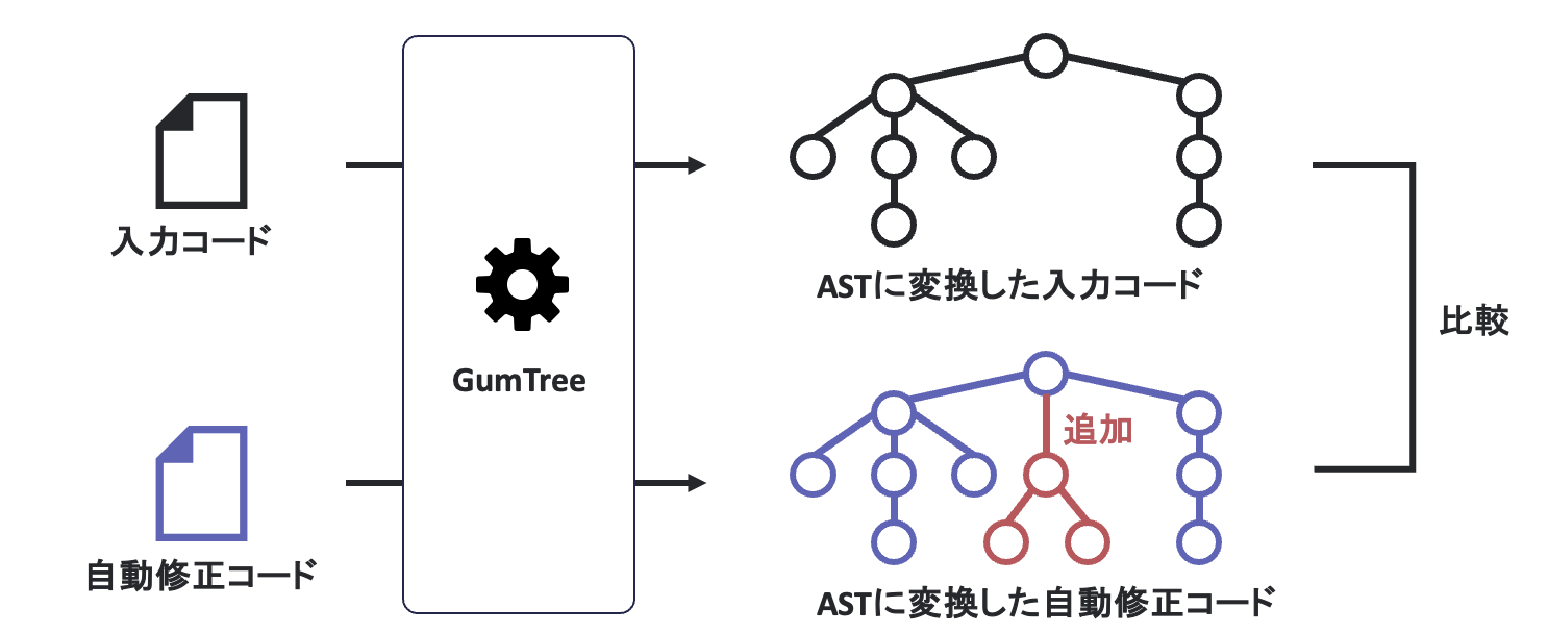
\includegraphics[width=1.0\linewidth]{@BSthesis2024_Akamatsu/Akamatsu_figs/AST.pdf}}
    \caption{変更箇所の特定方法の概略図}
    \label{fig:Insufficient_documentation}
\end{figure*}
提出されたメソッド($m_s$)と修正後のメソッド($m_r$)の変更箇所を特定するために,抽象構文木(AST: Abstract Syntax Tree)の差分分析を行った.差分分析にはGumTree\todo{参考文献}を使用し,以下の手順で変更箇所の特定を行った.

\begin{enumerate}
\item 提出されたメソッド($m_s$)と修正後のメソッド($m_r$)それぞれに対してASTを生成する.
\item GumTreeを用いて2つのAST間の差分を抽出する.GumTreeは以下の4種類の操作を特定する:
\begin{itemize}
\item 追加(INSERT):新しいノードの追加
\item 削除(DELETE):既存ノードの削除
\item 更新(UPDATE):ノードの値の更新
\item 移動(MOVE):ノードの位置の変更
\end{itemize}
\item 抽出された差分情報から,変更が行われた箇所とその種類を特定し,変更ノード数を算出する
\end{enumerate}
この手法により,変更差分を定量的に算出し,入力コード全体のノード数と比較する.

\section{分析結果}

\subsection {分析準備}

分析の準備として,以下の手順を行った

\begin{enumerate}
   \item データセットから入力コードのノード数と変更ノード数の外れ値を除去する.具体的には,それぞれの四分位範囲(IQR)を計算し,第1四分位数(Q1)から四分位範囲の1.5倍を引いた値より小さい値,または第3四分位数(Q3)に四分位範囲の1.5倍を加えた値より大きい値を外れ値として除去する.

   \item 入力コードのノード数とCodeBLEUスコアの関係性を分析するため,外れ値を除去した後のデータセットを入力コードのノード数に基づいて4つのグループに分割する.具体的には,ノード数の四分位数(Q1,Q2(中央値),Q3)を基準として,以下の4グループに分類する:
   \begin{itemize}
       \item グループ1:Q1未満のノード数
       \item グループ2:Q1以上Q2未満のノード数
       \item グループ3:Q2以上Q3未満のノード数
       \item グループ4:Q3以上のノード数
   \end{itemize}
\end{enumerate}

\subsection {分析1: グループ間のCodeBLEUスコアの分布の差異}

\begin{table}[h]
   \centering
   \caption{グループ間のマン・ホイットニーU検定のp値}
   \label{tab:mann-whitney}
   \begin{tabular}{l|cccc}
       \hline
       p値 & グループ1 & グループ2 & グループ3 & グループ4 \\
       \hline
       グループ1 & - & 9.60e-46 & 2.21e-83 & 1.00e-147 \\
       グループ2 & - & - & 3.29e-08 & 4.01e-37 \\
       グループ3 & - & - & - & 9.30e-14 \\
       グループ4 & - & - & - & - \\
       \hline
   \end{tabular}
\end{table}

各グループ間でCodeBLEUスコアの分布に統計的な差があるかを検証するため,マン・ホイットニーのU検定を実施した.有意水準は0.05に設定し,全てのグループの組み合わせで検定を行った結果,すべての組み合わせにおいてp値が有意水準を下回った(p \verb|<| 0.05).これは,入力コードのノード数の違いによってCodeBLEUスコアの分布が有意に異なることを示している.

表\ref{tab:mann-whitney}に示すように,全ての組み合わせにおいてp値は0.05を大きく下回っており,各グループ間のCodeBLEUスコアの分布には統計的に有意な差があることが確認された.

\subsection {分析2: 同一タスクにおけるコード量の影響}
\begin{figure}[h]
    \centering
    \fbox{\begin{minipage}{0.95\linewidth}
        \textbf{コード例1} \\
        \textbf{BLEU score: 0.750} \\
        \textbf{入力コードのノード数: 5} \\
        \textit{(赤色の部分は変更箇所を示す)} \\
        
        \ttfamily\small
public String getRpmRevision() \{\\
\hspace{4ex}return this.\textcolor{red}{rpmRevison};\\
\}

        \normalfont\hrule
        レビューコメント: typo above, be: return this.rpmRevision;
    \end{minipage}}

    \vspace{4mm}

    \fbox{\begin{minipage}{0.95\linewidth}
        \textbf{コード例2} \\
        \textbf{BLEU score: 0.996} \\
        \textbf{入力コードのノード数: 80} \\
        \textit{(赤色の部分は変更箇所を示す)} \\
        
        \ttfamily\small
public StringBuffer generate(\\
\hspace{4ex}final String packageName,\\
\hspace{4ex}final PackageElement packageElement,\\
\hspace{4ex}final String className,\\
\hspace{4ex}final Element element,\\
\hspace{4ex}final ProcessingEnvironment\\
\hspace{4ex}processingEnvironment) throws GenerationException \{\\
\hspace{4ex}final Messager messager =\\
\hspace{8ex}processingEnvironment.getMessager();\\
\hspace{4ex}Messager.printMessage(Diagnostic.Kind.NOTE,\\
\hspace{8ex}"Starting code \textcolor{red}{generation} for [" + className + "]");\\
\hspace{4ex}// ... (42行省略)\\
\}

        \normalfont\hrule
        レビューコメント: hey @pefernan , this one... is a typo
    \end{minipage}}
    \caption{同一タスク(タイプミス)における入力コード量の違いによるCodeBLEUスコアの比較}
    \label{fig:code-comparison}
\end{figure}

同じタイプの修正(タイプミス)に対して,入力コードの規模が異なる場合のCodeBLEUスコアを比較した.具体的には,変更ノード数が1で同一のタスク(タイプミスの修正)である2つのケースを分析した.その結果,入力コードのノード数が5の場合はCodeBLEUスコアが0.750であったのに対し,ノード数が80の場合は0.996と大幅に高いスコアを示した.これは,同じ種類の修正であっても,入力コードの規模が大きくなるとCodeBLEUスコアが高くなる傾向があることを示している

\subsection {分析3: ノード数別の修正規模とスコアの関係}
図\ref{fig:node-scores}に,入力コードのノード数によって分類した4つのグループにおける,変更ノード数とCodeBLEUスコアの分布を示す.横軸は変更ノード数を5刻みで区切ったグループを表し,縦軸は各グループにおけるCodeBLEUスコアの分布を箱ひげ図で表している.入力コードのノード数は3〜233の範囲を4分位で分割し,3〜25,25〜45,45〜75,75〜233の4グループとした.

\begin{figure}[h]
   \centering
   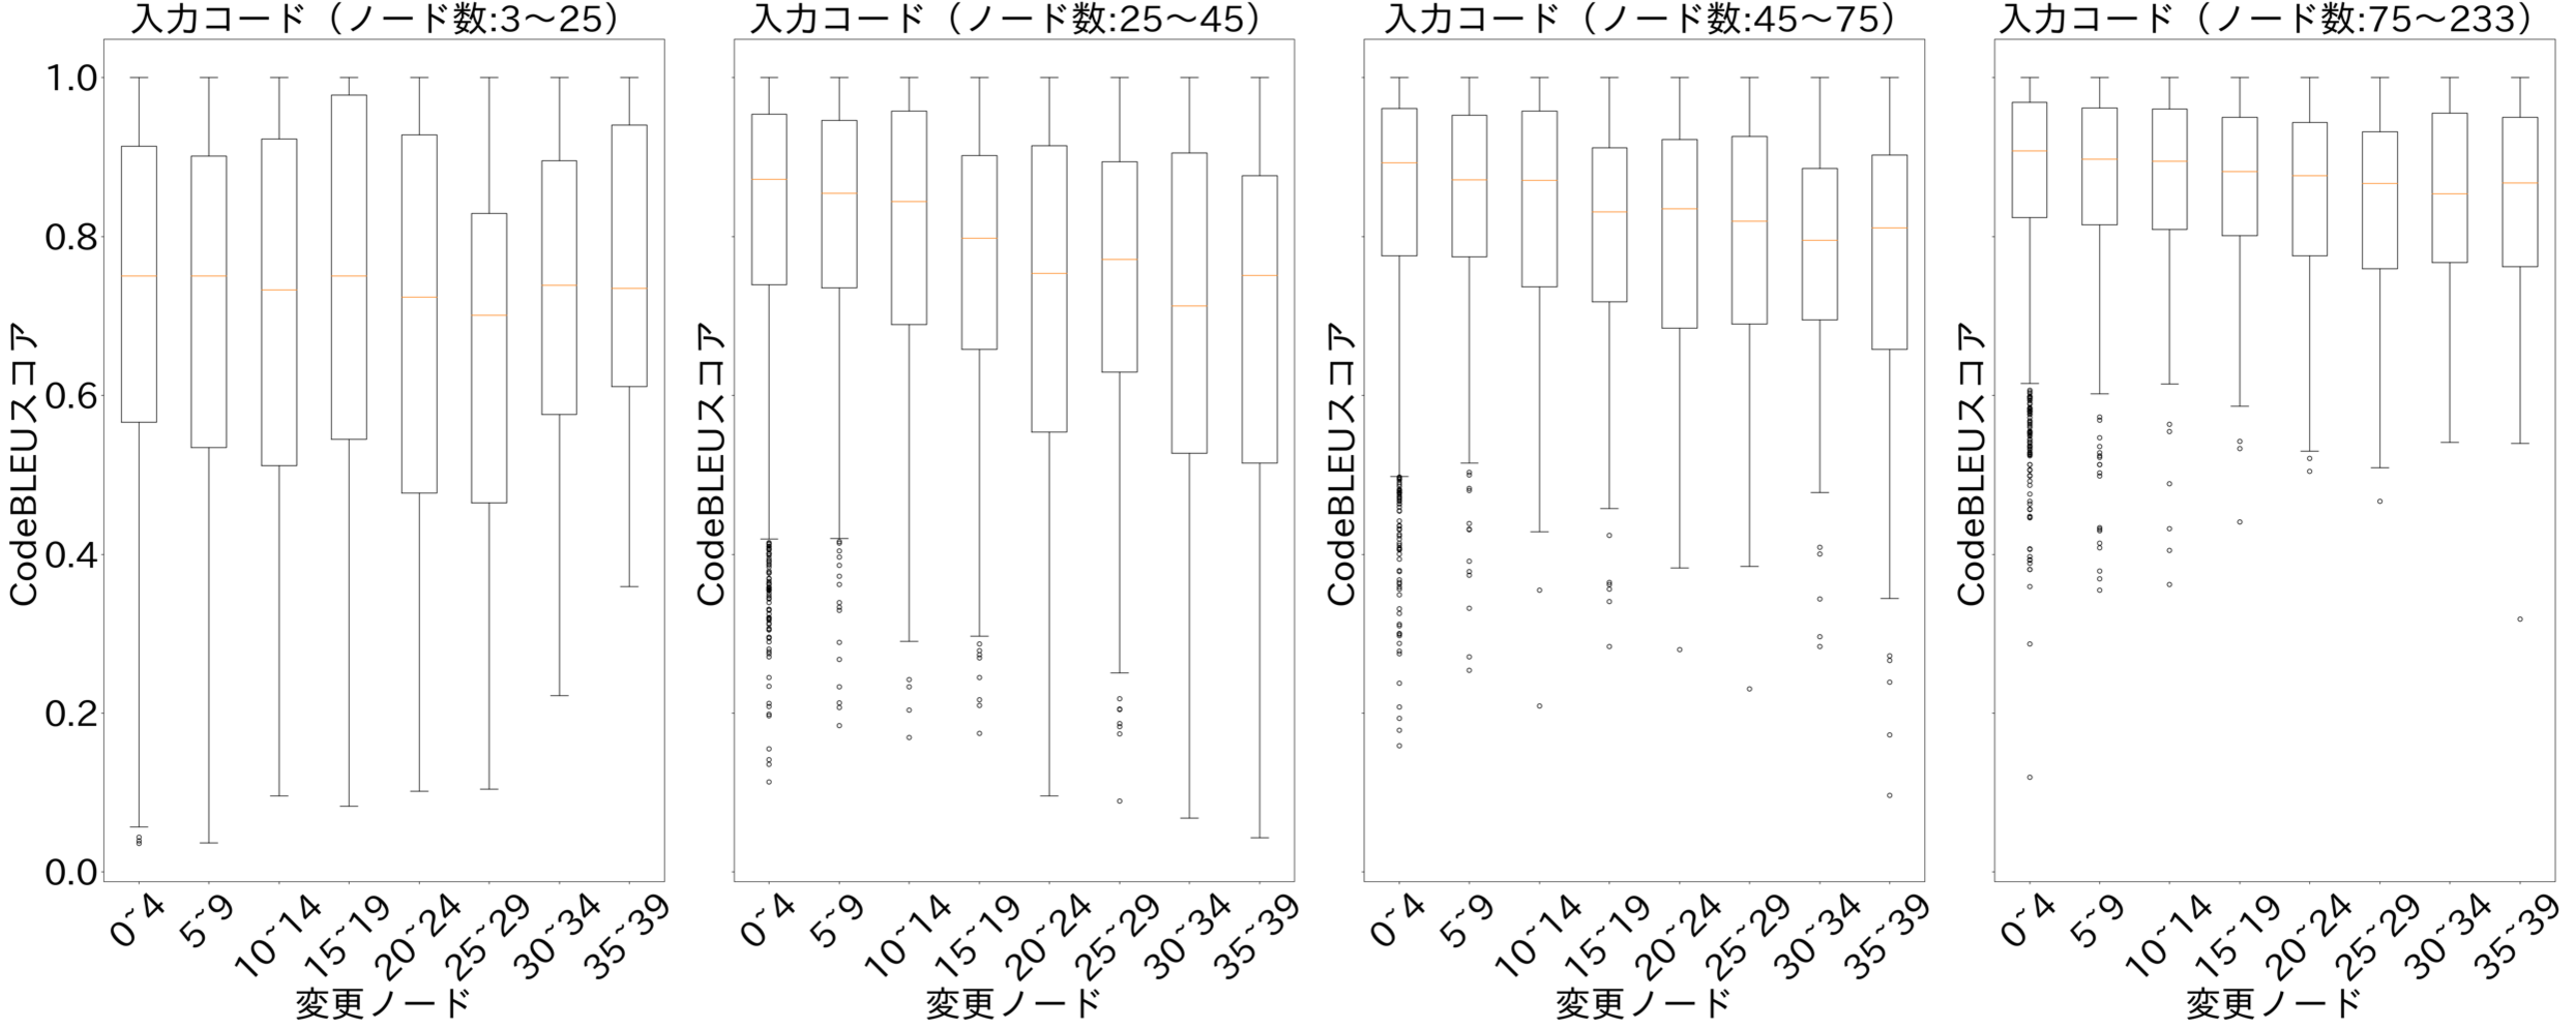
\includegraphics[width=1.0\linewidth]{@BSthesis2024_Akamatsu/Akamatsu_figs/nodescores.pdf}
   \caption{入力コードのノード数別のCodeBLEUスコアの分布}
   \label{fig:node-scores}
\end{figure}

特筆すべき分析結果として,以下の2点が挙げられる:

\begin{enumerate}
   \item 入力コードのノード数が75〜233(第3四分位数から最大値)の場合,変更ノード数が増加してもCodeBLEUスコアは0.8前後の高い値を維持している.これは,入力コード全体に対する変更部分の割合が相対的に小さくなるため,変更の規模に関わらず全体としての一致率が高くなってしまうことを示している.つまり,この範囲のノード数では,CodeBLEUスコアが修正の質を適切に評価できていない可能性がある.
   
   \item 入力コードのノード数が25〜45(第1四分位数から中央値)の場合,変更ノード数の増加に伴いCodeBLEUスコアが単調に減少する傾向が見られた.これは,コードの変更規模が大きくなるにつれて修正の難易度が上がり,生成精度が低下することを適切に反映している.この範囲のノード数では,CodeBLEUスコアが修正の質を適切に評価できていると考えられる.
\end{enumerate}

以上の分析結果から,CodeBLEUスコアを評価指標として使用する際は,入力コードのノード数が25〜45の範囲にあるケースを対象とすることで,より信頼性の高い評価が可能であることが示唆された.一方で,ノード数が75を超えるような大規模なコードに対しては,CodeBLEUスコアが実際の修正の質を反映していない可能性があり,評価指標としての使用には注意が必要である.これらの知見を踏まえ,以降の章では入力コードのノード数が25〜45の範囲にあるデータセットを用いて分析を行う.この範囲のデータセットを用いることで,CodeBLEUスコアによる評価の信頼性を確保し,より正確な分析結果を得ることを目指す.


\chapter{RQ1:\RQone}\label{chap:fig-tab-exp}

\section{概要}
本章では,レビューアが指摘したソースコードを自動生成するために必要なレビューコメントの情報の種類を明らかにする.
従来研究では,レビューコメントに基づくコード生成モデルの精度にばらつきがあることが示されているが,どのような情報の種類が自動生成の精度向上に寄与するかは詳細に分析されていない.レビューコメントに含まれる情報の種類が自動生成の精度に与える影響を明らかにするために,従来研究でGitHubおよびGerritから収集されたレビューコメントに対して情報の種類に関するラベル付けを行う.また,各情報の種類とコード生成モデルの精度の関係性を基に,レビューコメントに必要な情報の特徴をそれぞれ分析する.

\section{分析手法}


\subsection {データセット}
本分析では,3章と同じく従来研究で行われた分析結果を対象に分析を行った.

\begin{itemize}
    \item プロジェクト選定条件:
    \begin{itemize}
        \item プルリクエスト数が50件以上.
        \item 10人以上の貢献者および10個以上のスターを持つプロジェクト.
    \end{itemize}
    \item データ構造:
    \begin{itemize}
        \item 各データは以下の3つの要素で構成されている $\langle m_s, c_{nl}, m_r \rangle$:
        \begin{itemize}
            \item $m_s$: 提出されたメソッド.
            \item $c_{nl}$: レビュアーによる変更提案コメント.
            \item $m_r$: 修正後のメソッド,
        \end{itemize}
    \end{itemize}


\end{itemize}

\subsection{事前処理}
\begin{figure}[htbp]
    \centering
    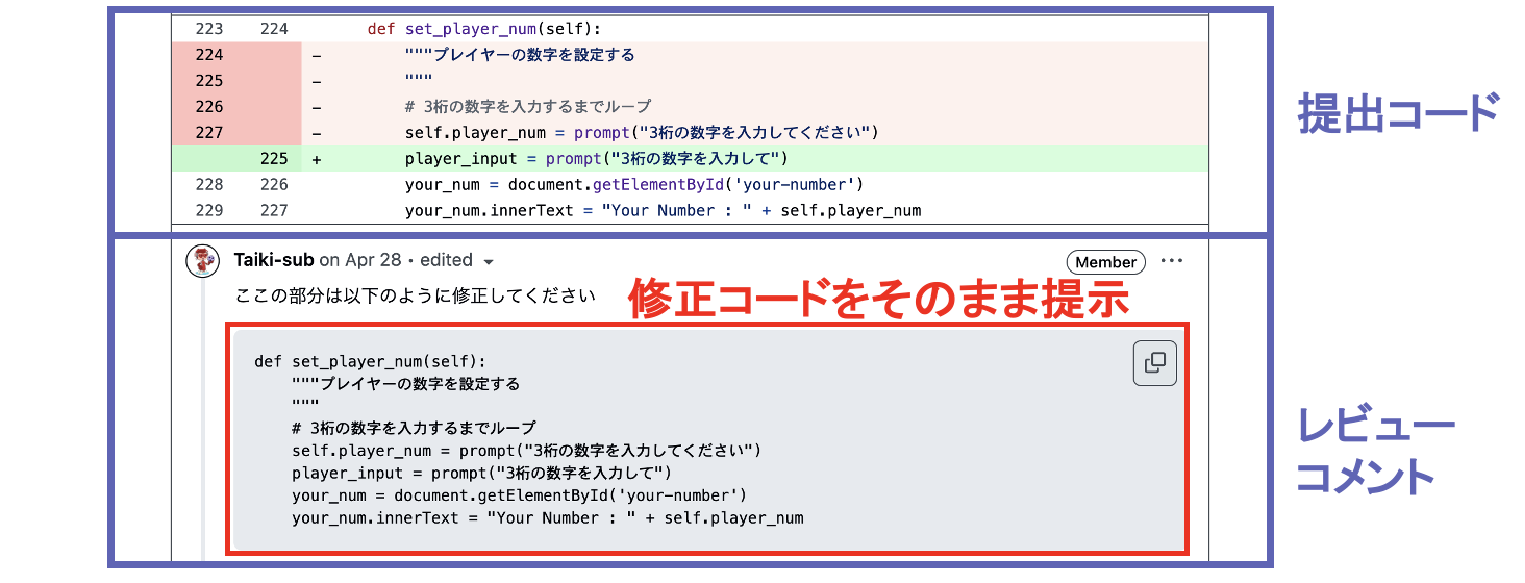
\includegraphics[width=0.8\linewidth]{@BSthesis2024_Akamatsu/Akamatsu_figs/review_comment.pdf}
    \caption{レビューアが修正コードを直接提供するレビューコメントの例}
    \label{fig:review-comment-example}
\end{figure}
分析に先立ち,収集したデータセットに対して以下の事前処理を行った.

3章で述べたように,CodeBLEUスコアを評価指標として使用する際は,入力コードのノード数が25〜45の範囲にあるケースを対象とすることで,より信頼性の高い評価が可能であることが示唆された.そのため,本分析では入力コードのノード数が25〜45の範囲にあるデータのみを抽出し,分析対象とした.これにより,CodeBLEUスコアによる評価の信頼性を確保し,より正確な分析結果を得ることを目指した.

次に,レビューコメントの内容を精査した.レビューコメントの中には,図\ref{fig:review-comment-example}に示すように,修正方法や修正理由の説明ではなく,修正後のコードそのものを提供している場合が存在する.このようなコメントは,レビューアが開発者の役割まで果たしているため,本研究の目的と逸脱している.またレビューアが意図した修正の背景や理由を理解することができず,レビューコメントから得られる情報の種類を適切に分析することができない.そのため,レビューコメントと修正コードとの文字列一致度を計算し,一致度が高いコメント,すなわち修正コードをそのまま含むコメントは分析対象から除外した.これにより,レビューアの意図や修正の理由が明確に記述されたコメントのみを分析対象とすることにした.

最後に,統計的な有意性を確保するためのサンプリングを行った.収集したデータセット全体(16,780件)に対して,統計的に有意な分析を行うために必要なサンプル数を算出した.具体的には,信頼水準95\%,許容誤差5\%の条件下で必要なサンプル数を計算し,375件のレビューコメントを無作為に抽出してラベル付けを行った..

これらの事前処理により,CodeBLEUスコアによる評価の信頼性を確保し,レビューコメントの本質的な情報を分析対象とし,かつ統計的な有意性を持つデータセットを準備することができた.


\subsection{ラベル付け}
レビューコメントに含まれる情報の種類を分析するため,各レビューコメントに対して2つの観点からラベル付けを行った.
1つ目の観点はコンテキストである.レビューアが指摘している修正の背景や目的を分類するため,以下の3つのカテゴリを設定した:
\begin{itemize}
\item リファクタリング:コードの可読性や保守性を向上させるための修正
\item バグ:プログラムの不具合や意図しない動作を修正
\item パフォーマンス:実行速度やメモリ使用量などの性能に関する修正
\end{itemize}
2つ目の観点は修正依頼方法である.レビューアがどのような形で修正を依頼しているかを分類するため,以下の3つのカテゴリを設定した:
\begin{itemize}
\item エラーの内容の提示:発生している問題や不具合の内容を説明
\item 再現方法の提示:問題が発生する条件や手順を説明
\item 具体的な修正方法の提示:どのように修正すべきかの具体的な方法を説明
\end{itemize}
なお,1つのレビューコメントに複数の情報が含まれる場合は,主たる情報に基づいてラベル付けを行った.

\section{結果}
レビューコメントの分析結果について,コンテキストと修正依頼方法の両観点から得られたCodeBLEUスコアの分布を図\ref{fig:context-score}に示す.
\begin{figure}[htbp]
\centering
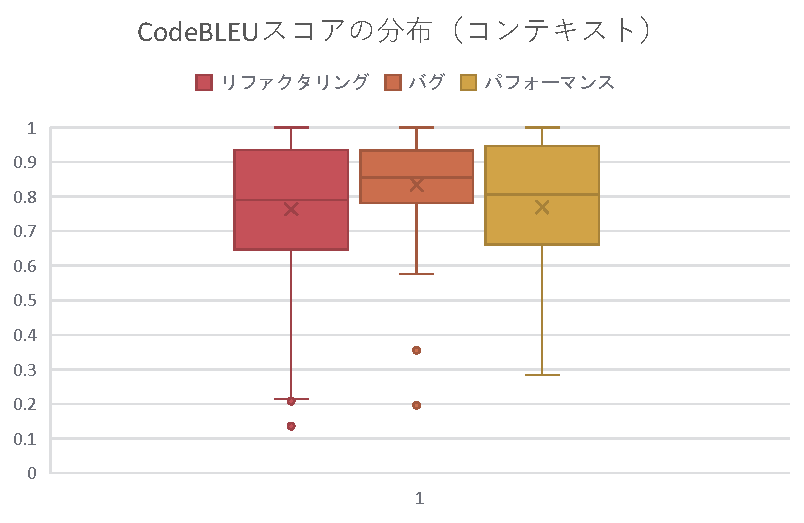
\includegraphics[width=0.8\linewidth]{@BSthesis2024_Akamatsu/Akamatsu_figs/rq1_result02.pdf}
\caption{コンテキストの種類別によるCodeBLEUスコアの分布比較}
\label{fig:context-score}
\end{figure}
まず,コンテキストの観点から見ると,リファクタリング,バグ,パフォーマンスの3種類のコンテキスト間でCodeBLEUスコアの分布に大きな差は見られなかった.各コンテキストのスコアの中央値はそれぞれ0.78,0.83,0.77程度であり,四分位範囲(IQR)も同程度の広がりを示している.特に,バグに関するコンテキストでは若干高いスコアを示す傾向があったものの,1種類のラベル間では,統計的有意差は確認されなかった(p > 0.05).このことから,修正の背景や目的の違いは,コード生成モデルの精度に大きな影響を与えないことが示唆された.また,全てのコンテキストにおいて,外れ値として0.2〜0.4程度の低いスコアを示すケースが観察されたが,これらは全体の5\%未満であり,モデルの一般的な性能を評価する上では無視できる範囲であると判断された.
一方,修正依頼方法の観点からの分析結果を図\ref{fig:method-score}に示す.
\begin{figure}[htbp]
\centering
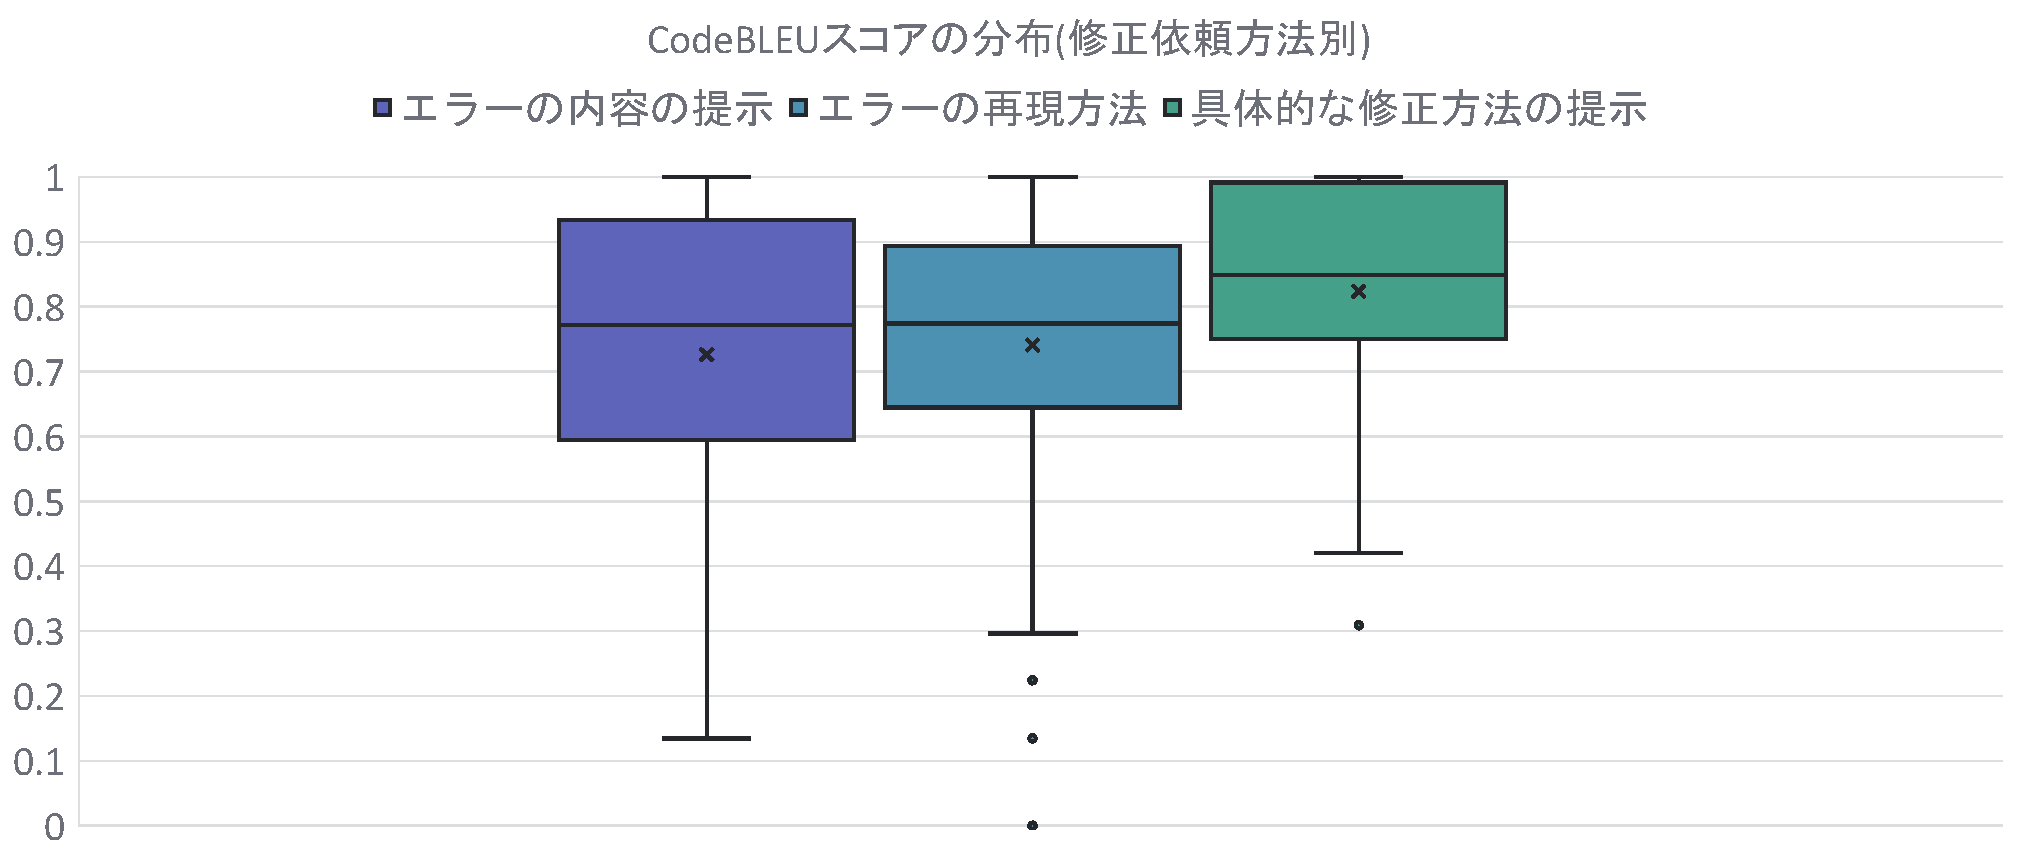
\includegraphics[width=0.8\linewidth]{@BSthesis2024_Akamatsu/Akamatsu_figs/rq1_result03.pdf}
\caption{修正依頼方法の違いによるCodeBLEUスコアの分布比較}
\label{fig:method-score}
\end{figure}
具体的な修正方法の提示が最も高いCodeBLEUスコアを示し(中央値:0.85,IQR:0.75-0.95),次いでエラーの再現方法(中央値:0.74,IQR:0.65-0.89),エラーの内容の提示(中央値:0.72,IQR:0.60-0.93)という順序となった.特筆すべき点として,具体的な修正方法を提示するコメントでは,スコアの分布がより上位に集中しており,外れ値も他の方法と比較して少ないことが確認された.これは,具体的な修正方法を提示することで,モデルがより安定して高精度なコード生成を実現できることを示唆している.
さらに,修正依頼方法とコンテキストを組み合わせた9つのカテゴリ(3×3)での分析結果を図\ref{fig:matrix-score}に示す.
\begin{figure}[htbp]
\centering
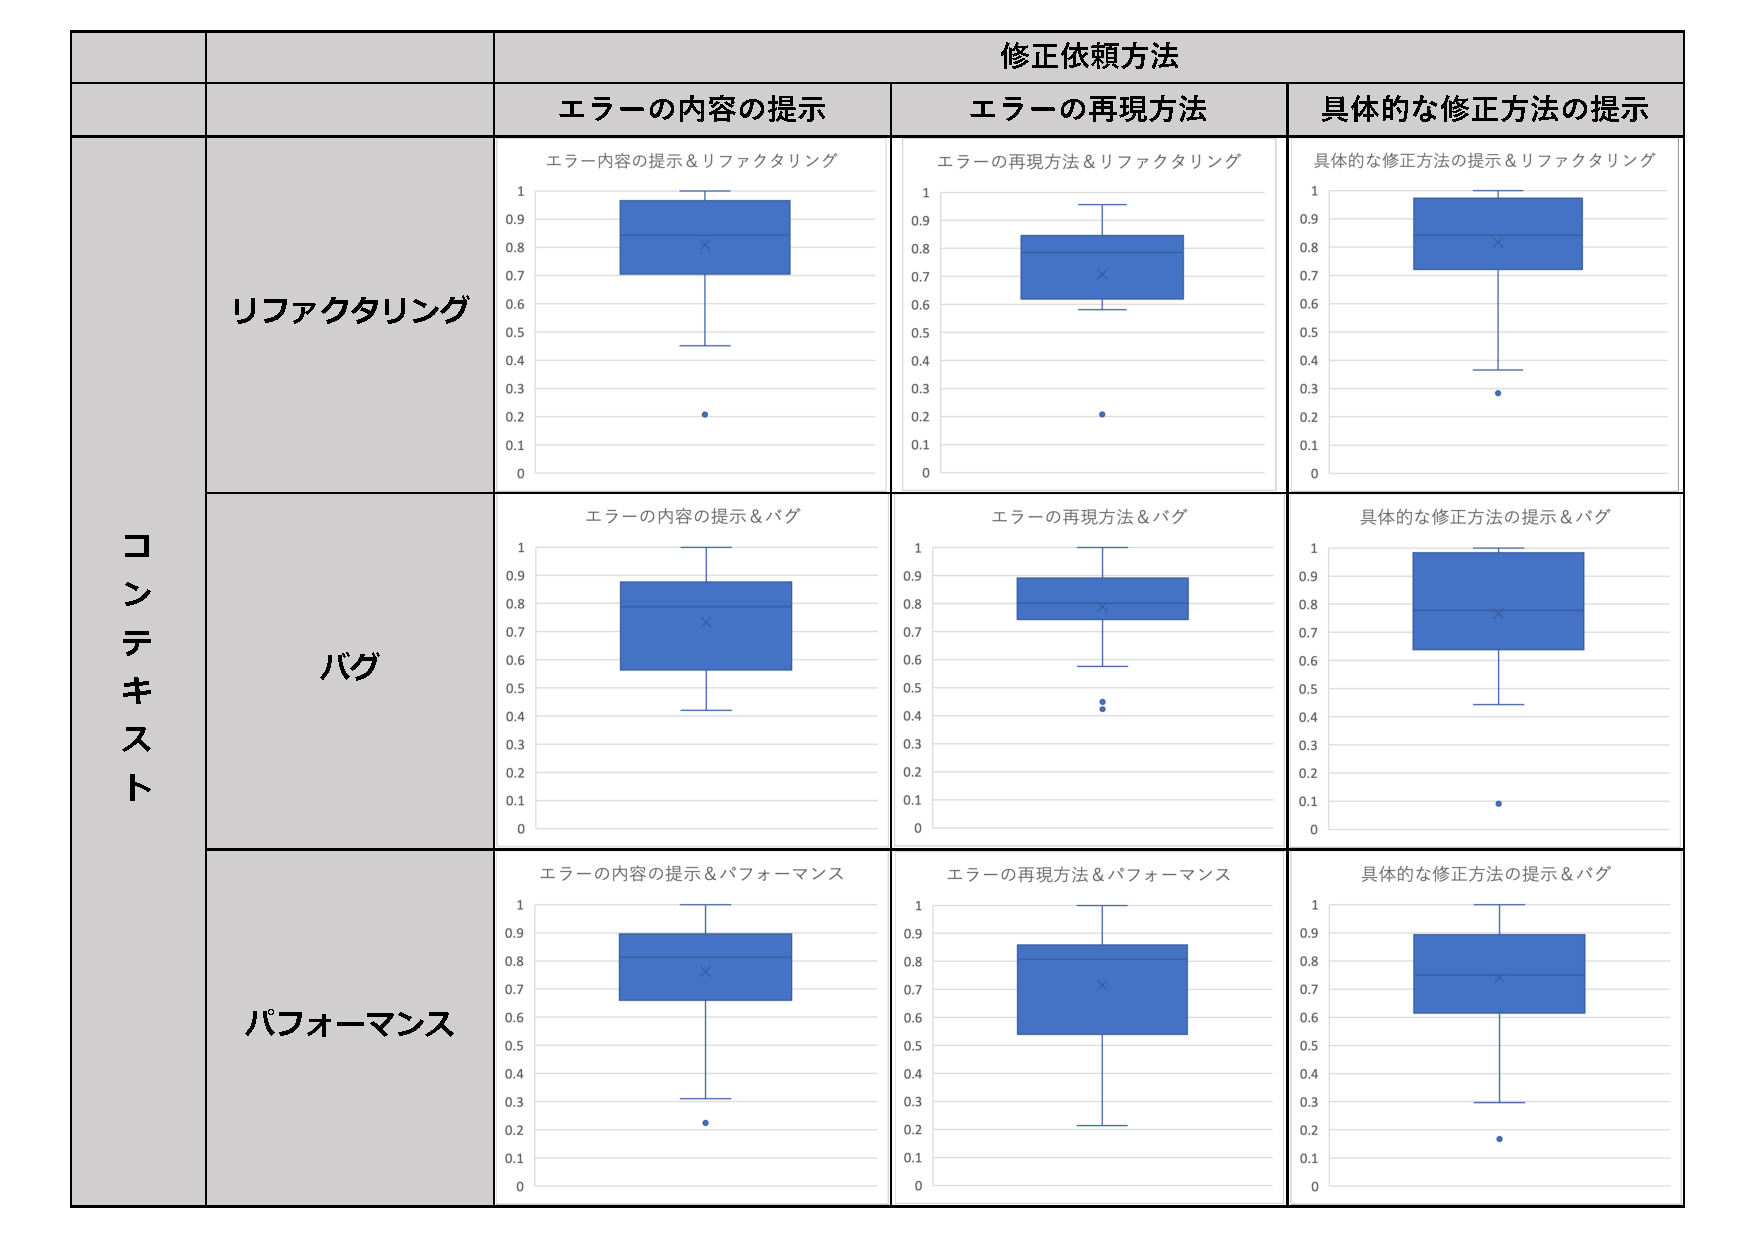
\includegraphics[width=0.9\linewidth]{@BSthesis2024_Akamatsu/Akamatsu_figs/rq1_result01.pdf}
\caption{修正依頼方法とコンテキストの組み合わせによるCodeBLEUスコアの分布}
\label{fig:matrix-score}
\end{figure}
例えば,「リファクタリング×具体的な修正方法の提示」や「バグ×エラーの再現方法」といった組み合わせごとにCodeBLEUスコアの分布を分析したが,カテゴリ間で統計的有意差は確認されなかった(p > 0.05).この結果は,コード生成の精度に最も影響を与えるのは修正依頼方法であり,コンテキストの違いによる影響は限定的であることを示している.また,この分析により,修正依頼方法の効果はコンテキストに依存せず,普遍的であることも示唆された.
これらの結果から,ソースコードを自動生成する際は,コンテキストの種類に関わらず,具体的な修正方法を提示するレビューコメントが最も効果的であることが明らかになった.また,エラーの再現方法や内容の提示だけでは,モデルが適切な修正を推論することが比較的困難であることも示された.


\chapter{RQ2:\RQtwo}\label{chap:fig-tab-exp}
\section{概要}
本章では,レビューアが指摘したソースコードを自動生成するために必要なレビューコメントの情報量を明らかにする.
従来研究では,レビューコメントに基づくコード生成モデルの精度にばらつきがあることが示されているが,自動生成の精度向上に必要な情報量については詳細な分析が行われていない.そこで本研究では,GitHubのPull Requestに含まれる追加情報(コミットメッセージ,ラベルなど)を用いてレビューコメントを段階的に拡張し,各段階での自動生成コードの精度を比較することで,効果的なコード生成に必要な情報量を定量的に分析する.


\section{データセット}
本分析では,GitHubから収集したPull Request(PR)とそれに関連するデータを対象とする.データ収集にあたっては,以下の条件を満たすPRを抽出した:
\begin{itemize}
\item マージされたJavaファイルを含むこと
\item マージされたJavaファイルに対するレビューコメントが存在すること
\item 対象のJavaファイルがそのPR内で変更されていること
\end{itemize}
データの収集では,GitHubのリポジトリをStar数の降順で検索し,上記条件を満たす1,808件のPRから,合計7,860件のレビューコメントを収集した.各PRについて,以下の情報を取得した:
\begin{itemize}
\item 自動コード修正モデルに入力する情報
\begin{itemize}
\item 変更前のJavaファイル:修正前の状態を示すソースコード
\item 変更後のJavaファイル:レビューコメントを受けて修正された後のソースコード
\item レビューコメント:レビューアによる指摘や提案内容
\end{itemize}
\item レビューコメントを拡張するためのPRに関するデータ
\begin{itemize}
\item PRタイトル:変更内容を要約したタイトル
\item PR Description:変更の詳細な説明や背景情報
\item ブランチ名:変更が行われたブランチの名称
\item ファイル名:対象となるJavaファイルの名称
\end{itemize}
\end{itemize}
第3章での分析結果から,CodeBLEUスコアによる評価の信頼性を確保するためには,入力コードのノード数が25〜45の範囲にあるデータを対象とすることが望ましい.そこで本分析では,収集した7,860件のレビューコメントから,入力コードのノード数が25〜45の範囲にあるデータのみを抽出し,最終的に7,079件のレビューコメントを分析対象とした.これにより,CodeBLEUスコアによる評価の信頼性を確保し,より正確な分析結果を得ることを目指す.

\section{分析手法}
レビューコメントに必要な情報量を分析するために,以下の手順で分析を行った.

\if0
\subsection{データ整形}
まず,収集したデータから分析に適した形式へのデータ整形を行った.具体的には,以下の処理を実施した:

\begin{itemize}
    \item レビューコメントが付与されている箇所を関数単位で抽出
    \item 自動修正ツールの入力形式に合わせて,Javaファイルとレビューコメントを結合
\end{itemize}
\fi
\subsection{レビューコメントの拡張}
GPTへの入力として,以下のコンテキスト情報を提供した:
\begin{itemize}
    \item 変更前のJavaファイル
    \item レビューコメント
    \item ファイルパス
    \item Pull Requestのタイトル
    \item Pull Requestの説明文
    \item ブランチ情報(変更元ブランチと変更先ブランチ)
\end{itemize}


\section {結果}

\chapter{考察}\label{chap:fig-tab-exp}


\chapter{妥当性への脅威}\label{chap:fig-tab-exp}

\section{内的妥当性}

\section {外的妥当性}

\chapter{おわりに}




\begin{acknowledgements}
.
\end{acknowledgements}


%%
%% 参考文献
%%
\begin{thebibliography}{99}

\bibitem{wusethesis}
  伊原彰紀,
  卒業論文スタイルファイル(和歌山大学システム工学部用),\\
  \url{https://github.com/fukuyasu/wuse_thesis}.

\bibitem{tex}
  Knuth, D.,
  Remarks to Celebrate the Publication of Computers \& Typesetting,
  TUGboat, Vol.7, No.2, pp.95--98, 1986.

\bibitem{latex}
  Lamport, L.,
  文書処理システム\LaTeXe{},
  ピアソン・エデュケーション,1999,
  \newblock{}阿瀬はる美 訳.

\bibitem{latex_j}
  奥村晴彦,\LaTeX{}入門 ---美文書作成のポイント---,技術評論社,1993.

\bibitem{latex2e}
  奥村晴彦,黒木裕介,[改定第6版] \LaTeXe~美文書作成入門,技術評論社,2013.

\bibitem{latexcomp}
  Goossens, M., Mittelbach, F. and Samarin, A.,
  The \LaTeX{}コンパニオン,アスキー出版局,1998,
  \newblock{}アスキー書籍編集部 監訳.

\bibitem{texwiki}
  \LaTeX 入門 --- \TeX{} Wiki,\\
  \url{https://texwiki.texjp.org/?LaTeX%E5%85%A5%E9%96%80},
  2021年12月3日閲覧.
\end{thebibliography}

%%%%%%%%%%%%%%%%%%%%%%%%%%%%%%%%%%%%%%%%%%%%%%%%%%%%%%%%%%%%%%%%%%%%%%%%

%%
%% 付録
%%
% \appendix
% 
% \chapter{サンプルプログラム}
% 
% プログラムリストや実行結果など,本論を補足する上で必要と思われるものが
% あれば付録として付ける.
% 
% {
% \footnotesize
% \begin{verbatim}
% #include <stdio.h>
% int main(void)
% {
%     printf("Hello, World!\n");
%     return 0;
% }
% \end{verbatim}
% }

%%%%%%%%%%%%%%%%%%%%%%%%%%%%%%%%%%%%%%%%%%%%%%%%%%%%%%%%%%%%%%%%%%%%%%%%

\end{document}
